\chapter{Construire un trou noir et le casse-tête de l’horizon}

\lectureoverview{Nous allons construire un trou noir à partir de trois éléments : le diagramme causal de l’espace-temps plat, le diagramme de Schwarzschild et le théorème de Birkhoff pour une coquille sphérique. Cette construction révèle qu’un horizon des événements est une frontière globale, qui peut commencer dans une région encore localement plate. Nous passerons ensuite de la géométrie causale à l’entropie et à la température de Hawking. Un thermomètre maintenu près de l’horizon devient arbitrairement chaud, tandis qu’un observateur en chute libre ne s’attend à aucune catastrophe locale. Pour conclure, nous nous demanderons ce qu’une expérience extérieure peut réellement établir sans provoquer la perturbation même qu’elle cherche à détecter.}

\section{Un trou noir à la température de l’espace vide}

Un devoir était censé être prévu : construire un trou noir et l’apporter en classe pour le montrer. Personne n’en avait à présenter, mais un calcul trouvé sur Wolfram a fourni un problème d’introduction plus doux. Quel rayon et quelle masse donneraient à un trou noir une température de Hawking proche de la température \(3\,\mathrm{K}\) du fond diffus cosmologique ?

\begin{classroomqa}
\audiencequestion{Qu’a-t-on calculé sur le site web ?\lecturetimestamp{00:00:39}}
\lecturerresponse{Le rayon d’un trou noir dont la température est d’environ \(3\,\mathrm{K}\). Le but n’est pas d’obtenir un calcul précis, mais d’estimer l’échelle physique.}
\end{classroomqa}

Un tel trou aurait momentanément la même température que son environnement, mais cet équilibre serait instable. Un trou noir de Schwarzschild a une capacité thermique négative. S’il devient légèrement plus chaud que le bain, il émet du rayonnement, perd de la masse et chauffe davantage. S’il devient légèrement plus froid, il absorbe du rayonnement, gagne de la masse et se refroidit davantage.\editorialnote{C’est l’argument précis de stabilité qui sous-tend la formulation volontairement approximative employée en classe. Un bain thermique canonique ne peut pas maintenir un trou noir de Schwarzschild isolé en équilibre stable.}

L’estimation commence par la longueur d’onde caractéristique du rayonnement \(3\,\mathrm{K}\).

\begin{classroomqa}
\audiencequestion{Quelle est la longueur d’onde d’un rayonnement à environ trois kelvins ?\lecturetimestamp{00:02:03}}
\lecturerresponse{Dans la salle, on a proposé un centimètre, \(21\) centimètres, et même \(10\) mètres, avant de retenir le domaine des micro-ondes. Pour le raisonnement, la réponse utile à l’ordre de grandeur était d’environ un centimètre, assez petit pour susciter les plaisanteries sur un four à micro-ondes et une boîte à pain.}
\end{classroomqa}

Le quantum de Hawking typique a une longueur d’onde comparable au rayon de Schwarzschild, à des facteurs numériques près :
\begin{equation}
\lambda_{\mathrm{H}}\sim R_s,
\qquad
R_s=\frac{2GM}{c^2}.
\label{eq:l05-scale}
\end{equation}
En prenant la valeur utilisée en classe \(\lambda_{\mathrm H}\sim1\,\mathrm{cm}\), on obtient \(R_s\sim1\,\mathrm{cm}\). Comme le rayon d’un trou noir d’une masse solaire est de quelques kilomètres et que \(R_s\) est proportionnel à \(M\), la masse correspondante est approximativement
\begin{equation}
M\sim10^{-5}M_\odot,
\label{eq:l05-rough-mass}
\end{equation}
soit une échelle planétaire. C’est pourquoi le cours aboutit à une estimation comparable à celle de la Terre.

\begin{classroomqa}
\audiencequestion{Est-ce compatible avec le résultat numérique obtenu avec Wolfram ?\lecturetimestamp{00:05:53}}
\lecturerresponse{Le résultat indiqué était plutôt proche de la masse de la Lune. Cela semblait faible par rapport à l’estimation grossière, mais dans les deux cas, le point essentiel est le même : ce n’est pas un objet qu’on pourrait porter dans sa poche.}
\end{classroomqa}

Le calcul détaillé des constantes explique l’écart. À partir de
\begin{equation}
T_H=\frac{\hbar c}{4\pi k_B R_s},
\end{equation}
on trouve, pour \(T_H=3\,\mathrm{K}\),
\begin{equation}
R_s\simeq6.1\times10^{-5}\,\mathrm{m},
\qquad
M\simeq4.1\times10^{22}\,\mathrm{kg}.
\label{eq:l05-three-kelvin}
\end{equation}
une masse lunaire plutôt que terrestre. La longueur d’onde des micro-ondes, le facteur \(4\pi\) et le choix de la longueur d’onde du corps noir considérée comme typique expliquent l’écart entre l’estimation rapide et la valeur numérique.\editorialnote{L’équation~\eqref{eq:l05-three-kelvin} rétablit les facteurs numériques omis dans l’estimation dimensionnelle du cours. Nous conservons cette estimation, car c’est la démarche suivie en classe.}

Le calcul a rempli son rôle. Nous voulons maintenant construire un trou noir, mathématiquement et par l’imagination. Les équations complètes du champ sont trop difficiles pour ce que nous cherchons à faire ici. Les schémas nous en donneront les éléments essentiels.

\section{Première étape : l’espace-temps plat}

Utilisons des coordonnées polaires centrées sur un observateur et supprimons les angles. Les coordonnées restantes sont \((t,r)\), avec \(r\geq0\). Un point de ce diagramme réduit n’est pas un point de l’espace-temps à quatre dimensions ; sauf en \(r=0\), il représente une sphère entière \(S^2\).

Les rayons lumineux radiaux se déplacent à \(45^\circ\). Un rayon entrant atteint l’origine, tandis qu’un rayon sortant la quitte dans l’autre direction nulle. Une transformation conforme permet de comprimer le demi-plan infini en un secteur de Penrose fini. Cette transformation n’est pas unique. Ses propriétés essentielles sont de ramener l’infini sur une frontière finie et de préserver les directions nulles radiales à \(45^\circ\). Pour reprendre l’expression employée au tableau, on écrase le diagramme.

\begin{figure}[htbp]
\centering
\includegraphics[width=0.68\textwidth]{lecture_05_figure_02.png}
\caption{La moitié supérieure de l’espace-temps de Minkowski compactifié en coordonnées radiales. Le bord vertical est \(r=0\), tandis que les familles de courbes se resserrent vers l’infini compactifié.}
\lectureframe{00:11:41.560}
\end{figure}

\begin{figure}[htbp]
\centering
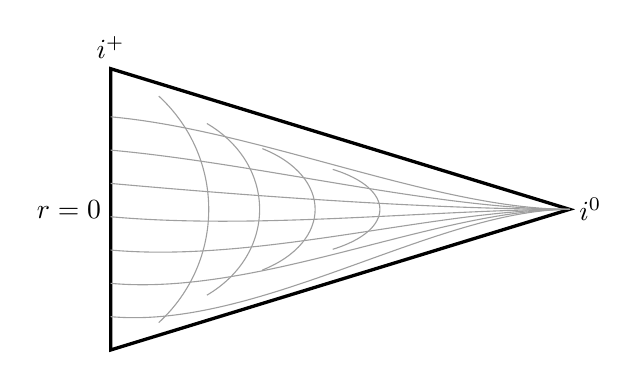
\begin{tikzpicture}[scale=0.94]
\coordinate (O) at (0,0);
\coordinate (P) at (0,3.8);
\coordinate (I) at (6.2,1.9);
\draw[very thick] (O)--(P)--(I)--cycle;
\foreach \y in {0.45,0.90,1.35,1.80,2.25,2.70,3.15} {
  \draw[gray!75] (0,\y) .. controls (2.0,\y-0.18) and (4.4,1.9) .. (I);
}
\draw[gray!75] (0.65,0.37) .. controls (1.55,1.20) and (1.55,2.60) .. (0.65,3.43);
\draw[gray!75] (1.30,0.74) .. controls (2.25,1.30) and (2.25,2.50) .. (1.30,3.06);
\draw[gray!75] (2.05,1.08) .. controls (3.00,1.46) and (3.00,2.34) .. (2.05,2.72);
\draw[gray!75] (3.00,1.36) .. controls (3.85,1.62) and (3.85,2.18) .. (3.00,2.44);
\node[left] at (0,1.9) {\(r=0\)};
\node[above] at (P) {\(i^+\)};
\node[right] at (I) {\(i^0\)};
\end{tikzpicture}
\caption{Version épurée du secteur supérieur. Les courbes représentent qualitativement les familles à valeur constante de \(r\) et de \(t\) ; elles ne constituent pas un réseau exact de coordonnées.}
\label{fig:l05-flat-wedge}
\end{figure}

Les lignes d’univers à \(r\) constant, verticales avant la compactification, s’incurvent et s’accumulent près de l’infini temporel futur. Les tranches à \(t\) constant se resserrent elles aussi en approchant de l’infini spatial. Ce resserrement est un effet de coordonnées, et non une compression physique de la matière.

La règle des \(45^\circ\) s’applique directement à la lumière radiale. Un rayon doté d’un moment cinétique peut éviter l’origine, atteindre une distance minimale non nulle, puis repartir vers l’extérieur. Loin de l’origine, sa projection paraît presque radiale ; ce n’est qu’au voisinage de son approche la plus proche que sa trajectoire réduite dans \((t,r)\) se courbe visiblement. La première étape est ainsi achevée.

\section{Deuxième étape : la solution éternelle de Schwarzschild}

La solution de Schwarzschild maximalement prolongée comprend deux losanges extérieurs, une région de trou noir futur et une région de trou blanc passé. Ses frontières ondulées supérieure et inférieure sont les singularités future et passée. Pour un trou noir formé par effondrement, nous abandonnerons bientôt la majeure partie de cette structure ; l’extérieur droit ordinaire est précisément la partie dont nous avons besoin.

\begin{figure}[htbp]
\centering
\includegraphics[width=0.72\textwidth]{lecture_05_figure_03.png}
\caption{Diagramme de Schwarzschild éternel, avec l’extérieur ordinaire et son réseau de coordonnées schématique à droite.}
\lectureframe{00:16:55.975}
\end{figure}

\begin{figure}[htbp]
\centering
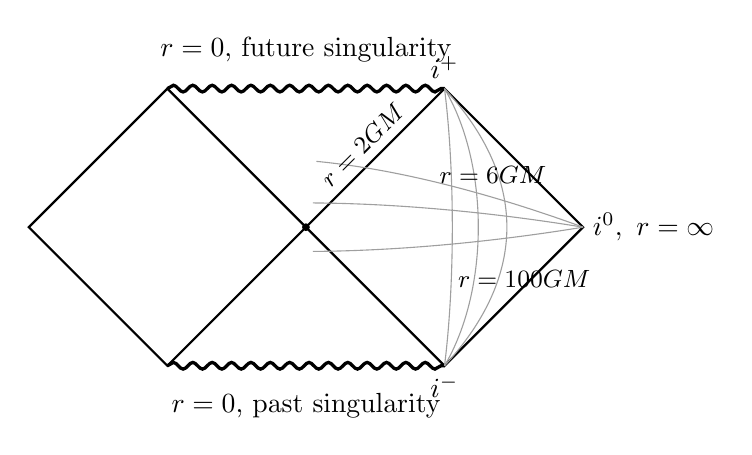
\begin{tikzpicture}[scale=0.88]
\coordinate (C) at (0,0);
\coordinate (TL) at (-2.0,2.0);
\coordinate (L) at (-4.0,0);
\coordinate (BL) at (-2.0,-2.0);
\coordinate (TR) at (2.0,2.0);
\coordinate (R) at (4.0,0);
\coordinate (BR) at (2.0,-2.0);
\draw[thick] (C)--(TL)--(L)--(BL)--(C);
\draw[thick] (C)--(TR)--(R)--(BR)--(C);
\draw[very thick,decorate,decoration={snake,amplitude=1.2pt,segment length=7pt}] (TL)--(TR);
\draw[very thick,decorate,decoration={snake,amplitude=1.2pt,segment length=7pt}] (BL)--(BR);
\draw[gray!75] (TR) .. controls (2.15,0.8) and (2.15,-0.8) .. (BR);
\draw[gray!75] (TR) .. controls (2.65,0.9) and (2.65,-0.9) .. (BR);
\draw[gray!75] (TR) .. controls (3.20,0.7) and (3.20,-0.7) .. (BR);
\draw[gray!75] (0.15,0.95) .. controls (1.5,0.82) and (2.9,0.40) .. (R);
\draw[gray!75] (0.10,0.35) .. controls (1.5,0.34) and (2.9,0.18) .. (R);
\draw[gray!75] (0.10,-0.35) .. controls (1.5,-0.34) and (2.9,-0.18) .. (R);
\fill (C) circle (1.6pt);
\node[above] at (TR) {\(i^+\)};
\node[below] at (BR) {\(i^-\)};
\node[right] at (R) {\(i^0,\ r=\infty\)};
\node[above] at (0,2.25) {\(r=0\), future singularity};
\node[below] at (0,-2.25) {\(r=0\), past singularity};
\node[rotate=45,above,font=\small] at (1.0,1.0) {\(r=2GM\)};
\node[font=\small] at (2.70,0.75) {\(r=6GM\)};
\node[font=\small] at (3.15,-0.75) {\(r=100GM\)};
\end{tikzpicture}
\caption{À grand rayon, l’extérieur droit ressemble au secteur plat. Son bord intérieur nul est \(r=2GM\) lorsque \(c=1\) ; les autres rayons indiqués sont des exemples schématiques.}
\label{fig:l05-eternal-schwarzschild}
\end{figure}

Loin du trou noir, l’extérieur ressemble de plus en plus à l’espace plat compactifié. Des lignes telles que \(r=6GM\) et \(r=100GM\) se rapprochent du comportement de lignes d’univers à rayon constant ordinaire. La frontière intérieure de l’extérieur se trouve à
\begin{equation}
r=2GM
\end{equation}
dans les unités \(c=1\).

Près du centre, la comparaison avec l’espace plat ne tient plus. Dans l’espace de Minkowski, un rayon radial atteint \(r=0\) et ressort de l’autre côté physique. À l’intérieur de Schwarzschild, un rayon orienté vers le futur ne rebondit pas. Il se termine sur la singularité de genre espace en \(r=0\). C’est cette différence causale que la construction par effondrement doit préserver.

\section{Le théorème qui permet d’assembler les morceaux}

L’ingrédient manquant apparaît d’abord en gravitation newtonienne. Pour une distribution de masse à symétrie sphérique, la loi de Gauss donne
\begin{equation}
\oint\mathbf g\cdot d\mathbf A=-4\pi G M_{\mathrm{enc}},
\end{equation}
et donc
\begin{equation}
\mathbf g(r)=-\frac{G M_{\mathrm{enc}}(r)}{r^2}\,\hat{\mathbf r}.
\label{eq:l05-shell-theorem}
\end{equation}
La matière située à l’extérieur de la sphère de rayon \(r\) ne contribue pas au champ net en ce point. Pour une coquille creuse de masse totale \(M\),
\begin{equation}
\mathbf g=
\begin{cases}
0, & r<R_{\mathrm{shell}},\\[3pt]
-\dfrac{GM}{r^2}\hat{\mathbf r}, & r>R_{\mathrm{shell}}.
\end{cases}
\end{equation}

Le théorème de Birkhoff en est l’équivalent relativiste. Toute région du vide à symétrie sphérique est localement une région de Schwarzschild, caractérisée par un paramètre de masse constant. L’intérieur vide d’une coquille sphérique a un paramètre de masse nul et est localement minkowskien ; l’extérieur a un paramètre de masse \(M\) et est une région de Schwarzschild :
\begin{equation}
\begin{aligned}
M_{\mathrm{enc}}&=0 && \text{inside the shell},\\
M_{\mathrm{enc}}&=M && \text{outside the shell}.
\end{aligned}
\label{eq:l05-birkhoff}
\end{equation}
Ce résultat reste utile lorsque la coquille est en mouvement, car les régions de vide de part et d’autre conservent leur symétrie sphérique.

\editorialnote{Dire que l’intérieur est plat est une affirmation locale. Une coquille statique peut modifier la normalisation de la coordonnée temporelle intérieure, même si la courbure intérieure est nulle. Pour une coquille en mouvement ou une coquille nulle, il faut raccorder les deux métriques du vide à travers la coquille ; cette construction idéalisée est un raccordement par une coquille mince, étroitement apparenté à la géométrie de Vaidya entrante. Aucune de ces précisions ne modifie l’argument causal d’assemblage utilisé ici.}

Pour se représenter la situation en laboratoire, imaginons une sphère densément couverte de lasers synchronisés, comme dans une grande installation de confinement inertiel, tous déclenchés simultanément vers l’intérieur. Dans l’idéalisation, il n’y a pas d’appareillage, seulement une coquille lumineuse parfaitement sphérique. La coquille transporte une énergie \(E\), si bien que le paramètre de masse extérieur vaut
\begin{equation}
M=\frac{E}{c^2},
\end{equation}
ou simplement \(E=M\) en unités naturelles. Comme la coquille se déplace à la vitesse de la lumière, elle est représentée par une ligne nulle entrante dans le diagramme réduit. Chaque point de cette ligne représente un front d’onde sphérique entier, et non la trajectoire d’un photon.

\section{Raccorder l’espace-temps de l’effondrement}

Partons de l’espace-temps plat et traçons la coquille nulle entrante. La région à l’intérieur de la coquille est correcte : d’après le théorème de Birkhoff, elle est plate. La région extérieure est incorrecte, car la géométrie de Schwarzschild de l’extérieur doit déjà tenir compte de la masse totale de la coquille.

Traçons maintenant la même coquille dans le diagramme de Schwarzschild éternel. La région située à l’extérieur de la coquille y est correcte. Le trou blanc, le second extérieur et la partie inappropriée de l’intérieur du trou noir ne conviennent pas à un effondrement commençant dans un espace vide ordinaire : effaçons-les.

\begin{figure}[htbp]
\centering
\includegraphics[width=0.72\textwidth]{lecture_05_figure_05.png}
\caption{La coquille nulle, en rouge, tracée sur le diagramme de Schwarzschild pendant qu’on isole la portion correcte de l’extérieur.}
\lectureframe{00:32:00.000}
\end{figure}

Dans la portion plate, la coquille atteint \(r=0\). Dans la portion de Schwarzschild, elle atteint le début de la singularité future. Il s’agit du même point terminal. En raccordant l’intérieur plat à l’extérieur de Schwarzschild le long de la coquille, on obtient l’espace-temps le plus simple décrivant la formation d’un trou noir.

\begin{classroomqa}
\audiencequestion{Au point de raccordement supérieur gauche, le point terminal dans l’espace plat est-il vraiment le même que le point du côté de Schwarzschild ?\lecturetimestamp{00:34:50}}
\lecturerresponse{Oui. La coquille de l’espace plat se réduit à \(r=0\), et la singularité de Schwarzschild se trouve également en \(r=0\). Les deux points identifiés ont la même signification géométrique : la sphère s’est réduite à une taille nulle.}
\end{classroomqa}

\begin{figure}[htbp]
\centering
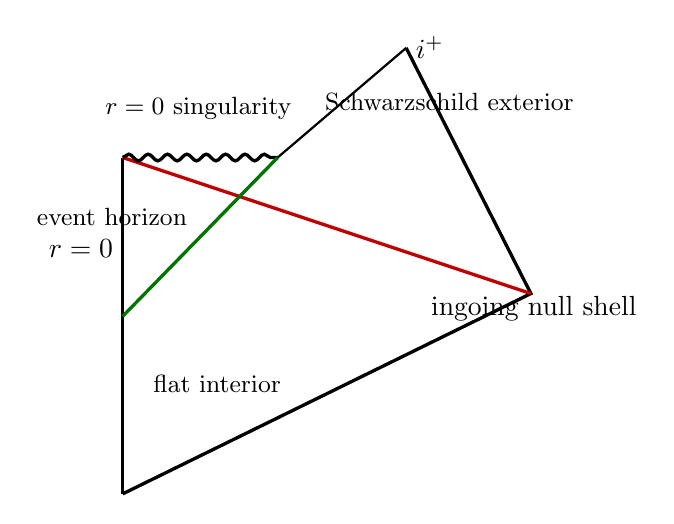
\begin{tikzpicture}[scale=0.96]
\coordinate (A) at (0,-2.8);
\coordinate (B) at (0,1.65);
\coordinate (C) at (2.05,1.65);
\coordinate (D) at (5.4,-0.15);
\coordinate (E) at (3.75,3.10);
\coordinate (H0) at (0,-0.45);
\draw[very thick] (A)--(B);
\draw[very thick] (A)--(D)--(E);
\draw[very thick,red!75!black] (D)--(B);
\draw[very thick,decorate,decoration={snake,amplitude=1.2pt,segment length=7pt}] (B)--(C);
\draw[very thick,green!45!black] (H0)--(C);
\draw[thick] (C)--(E);
\node[left] at (0,0.45) {\(r=0\)};
\node[below right] at (3.95,-0.05) {ingoing null shell};
\node[font=\small] at (1.25,-1.35) {flat interior};
\node[font=\small,anchor=west] at (2.55,2.38) {Schwarzschild exterior};
\node[above,font=\small] at (1.0,2.02) {\(r=0\) singularity};
\node[above left,font=\small] at (0.98,0.62) {event horizon};
\node[right] at (E) {\(i^+\)};
\end{tikzpicture}
\caption{Géométrie de l’effondrement. La coquille rouge relie un intérieur plat à un extérieur de Schwarzschild. L’horizon des événements vert commence plus tôt dans la région plate et se termine à la frontière future de la région du trou noir.}
\label{fig:l05-collapse}
\end{figure}

Cette construction répond à une question que la solution éternelle laissait en suspens. Un trou noir formé par effondrement n’a ni trou blanc passé ni second univers asymptotique. Il a tout de même une singularité future.

\section{L’horizon est une frontière globale}

L’ancienne étiquette \(r=2GM\) désignait l’horizon dans la géométrie stationnaire de Schwarzschild, mais elle ne donne pas la définition nécessaire en espace-temps dynamique.

\begin{definition}L’horizon des événements futur est la frontière de l’ensemble des événements qui peuvent envoyer un signal causal orienté vers le futur jusqu’à l’infini nul futur.\end{definition}

Sur le diagramme de l’effondrement, suivons le rayon lumineux sortant qui échoue de justesse à s’échapper. Les rayons juste à l’extérieur atteignent l’infini ; ceux qui sont juste à l’intérieur se terminent sur la singularité. Cette ligne de séparation est le véritable horizon.

\begin{figure}[htbp]
\centering
\includegraphics[width=0.72\textwidth]{lecture_05_figure_06.png}
\caption{Construction complète au tableau. La coquille entrante est rouge et l’horizon des événements est vert ; une partie de la ligne verte se trouve dans la région encore plate, sous la coquille.}
\lectureframe{00:39:10.000}
\end{figure}

Le trait surprenant de cette construction s’impose alors : l’horizon remonte jusqu’à une région que la coquille n’a pas encore atteinte. La géométrie y est localement plate, et un observateur qui franchit cette ligne ne détecte ni impulsion de courbure, ni mur, ni éclair. Pourtant, il ne peut déjà plus atteindre l’infini, car la coquille future fermera toutes les voies d’évasion possibles. Les horizons des événements sont téléologiques en ce sens précis, global : pour les situer, il faut connaître l’ensemble du futur de l’espace-temps.\editorialnote{Aucune expérience locale ne permet de déterminer qu’on vient de franchir un horizon des événements lisse. D’autres notions, comme celles d’horizon apparent ou d’horizon piégeant, sont plus locales et ne coïncident pas nécessairement avec l’horizon des événements pendant l’effondrement.}

L’analogie de la bonde met en évidence l’idée causale. Imaginons un rameur près d’une bonde bouchée, sur un lac immobile. Si le bouchon restait en place pour toujours, le rameur pourrait s’en aller. Mais si quelqu’un est certain de le retirer, le courant qui apparaîtra ensuite pourrait rendre la fuite impossible, alors même que l’eau ne bouge pas encore. Une chute du Niagara gelée illustre la même idée : l’eau calme ne garantit pas qu’une voie vers la sécurité restera ouverte.

\begin{classroomqa}
\audiencequestion{Le bouchon est-il retiré parce que la coquille de lumière devient de plus en plus concentrée ?\lecturetimestamp{00:43:13}}
\lecturerresponse{La concentration forme le trou noir, mais l’analogie de la bonde sert ici à illustrer une idée plus restreinte : on peut déjà se trouver au-delà du point de non-retour avant qu’un phénomène local spectaculaire ne se produise.}
\end{classroomqa}

\subsection{Un horizon constitué de sphères qui grandissent}

Chaque point de l’horizon réduit représente une \(S^2\). À l’origine de l’horizon, cette sphère a une aire nulle. En remontant le long de l’horizon, elle grandit jusqu’à ce que son rayon aréolaire atteigne
\begin{equation}
R_s=\frac{2GM}{c^2}.
\end{equation}
Elle conserve cette taille pour un trou noir stationnaire et grandit à nouveau si davantage d’énergie tombe dans le trou noir.

\editorialnote{Dans le diagramme idéalisé de l’effondrement sphérique, les génératrices de l’horizon se rencontrent en un point de formation, ou pli, sur \(r=0\). C’est cette sphère limite qui a une aire nulle ; cela ne signifie pas qu’un horizon de Schwarzschild de taille finie se réduit soudainement à un point.}

\subsection{Ce que l’observateur lointain peut reconstituer}

La longue discussion qui suit distingue l’observateur déjà à l’intérieur de l’horizon global de l’histoire qui l’y a conduit.

\begin{classroomqa}
\audiencequestion{Quel est le statut de la personne piégée avant l’arrivée de la coquille ? Du point de vue de l’observateur lointain, cette personne est-elle à l’extérieur de l’horizon ?\lecturetimestamp{00:44:03}}
\lecturerresponse{Non. Une fois que sa ligne d’univers se trouve derrière l’horizon des événements, son avenir la conduit à la singularité et aucun nouveau signal émis par elle ne parvient à l’observateur lointain. Mais cette personne n’a pas commencé à exister à cet endroit. Des particules antérieures, des ancêtres ou d’autres formes d’énergie précurseurs sont entrés depuis une région visible.}
\end{classroomqa}

L’observateur lointain peut donc voir la matière précurseur s’approcher de l’horizon sans jamais recevoir de signal provenant de l’autre côté. Il n’y a pas de contradiction à voir à travers la coquille entrante : elle est faite de lumière, et l’observateur peut aussi voir la coquille elle-même et déduire qu’un trou noir s’est formé.

\begin{classroomqa}
\audiencequestion{La ligne de visée traverse-t-elle la coquille en effondrement, et l’observateur extérieur peut-il encore savoir que le trou noir s’est formé ?\lecturetimestamp{00:46:51}}
\lecturerresponse{Oui. L’observateur voit la coquille entrante et peut recevoir de la lumière dont le trajet la traverse, tant que cette lumière peut encore s’échapper. Ce qui paraît étrange, c’est que la matière précurseur s’approche de l’horizon nouvellement déterminé avant même que la coquille atteigne le centre.}
\end{classroomqa}

\begin{classroomqa}
\audiencequestion{Est-ce dans la continuité de l’idée selon laquelle, vue de l’extérieur, la matière semble avoir été comprimée sur l’horizon ?\lecturetimestamp{00:47:49}}
\lecturerresponse{Oui. Dans la description extérieure, elle reste associée à l’horizon et subit un décalage vers le rouge toujours plus important, jusqu’à ce que le processus quantique ultérieur d’évaporation du trou noir change la donne.}
\end{classroomqa}

Cette description extérieure mène au sujet suivant. Si l’information semble plaquée sur une surface bidimensionnelle, il est moins surprenant que l’entropie du trou noir soit proportionnelle à l’aire de cette surface.

\section{Entropie et température mesurée depuis l’infini}

Près d’un grand horizon, nous pouvons remplacer la surface sphérique par un plan local, comme dans l’approximation de la Terre plate à l’échelle d’un petit laboratoire. Nous réunissons alors deux résultats de la discussion précédente :
\begin{equation}
\begin{aligned}
S_{\mathrm{BH}}&\propto A_H,\\
\Delta A_H&\sim \ell_P^2
\quad\text{per added bit, schematically}.
\end{aligned}
\end{equation}
La règle mnémotechnique d’un bit par aire de Planck exprime la loi d’échelle en aire ; elle n’en constitue pas une dérivation microscopique.

La température de Hawking mesurée loin d’un trou noir de Schwarzschild est
\begin{equation}
T_H=\frac{\hbar c^3}{8\pi GMk_B}.
\label{eq:l05-hawking}
\end{equation}
Avec \(R_s=2GM/c^2\),
\begin{equation}
T_H=\frac{\hbar c}{4\pi k_B R_s}.
\label{eq:l05-hawking-radius}
\end{equation}
Ainsi, plus les trous noirs sont grands, plus ils sont froids.

\begin{classroomqa}
\audiencequestion{La température peut-elle dépendre de la position ?\lecturetimestamp{00:52:43}}
\lecturerresponse{Dans la conversation courante, c’est manifestement possible : New York et Stanford n’ont pas nécessairement la même température. La question plus précise concerne un système en équilibre thermique gravitationnel. Dans ce cas, les températures locales indiquées par les thermomètres peuvent varier avec l’altitude, alors que la température d’équilibre redécalée vers le rouge reste constante.}
\end{classroomqa}

On mesure la température à partir des énergies cinétiques locales. Dans une atmosphère diluée au-dessus d’une Terre chauffée, les molécules perdent de l’énergie cinétique en montant et en gagnent en descendant. Les photons sont décalés vers le rouge en remontant et vers le bleu en redescendant. Un thermomètre placé en bas et un autre placé en haut ne sont donc pas nécessairement étalonnés sur la même échelle d’énergie locale.

Dans un espace-temps statique, la relation d’équilibre est
\begin{equation}
T_{\mathrm{loc}}(r)\sqrt{-g_{tt}(r)}=T_\infty,
\label{eq:l05-tolman}
\end{equation}
C’est la loi de Tolman. La température de Hawking dans l’équation~\eqref{eq:l05-hawking} est \(T_\infty\), la température normalisée à l’infini.

\section{L’atmosphère statique chaude près de l’horizon}

Soit \(\rho\) la distance propre mesurée vers l’extérieur depuis l’horizon. Au voisinage d’un grand horizon de Schwarzschild, l’équation~\eqref{eq:l05-tolman} devient
\begin{equation}
k_B T_{\mathrm{loc}}(\rho)
\simeq\frac{\hbar c}{2\pi\rho},
\label{eq:l05-local-temperature-si}
\end{equation}
ou, dans les unités \(c=\hbar=k_B=1\),
\begin{equation}
T_{\mathrm{loc}}(\rho)=\frac{1}{2\pi\rho}.
\label{eq:l05-local-temperature}
\end{equation}

\begin{figure}[htbp]
\centering
\includegraphics[width=0.72\textwidth]{lecture_05_figure_07.png}
\caption{La température de Hawking asymptotique et la température locale près de l’horizon \(T(\rho)=1/(2\pi\rho)\) inscrites au tableau.}
\lectureframe{01:02:40.000}
\end{figure}

Un minuscule thermomètre maintenu à \(\rho\) constant par un câble indique une température qui augmente à mesure qu’on l’abaisse. Un atome maintenu dans cette atmosphère statique s’excite, puis s’ionise, puis se dissocie ; à des énergies locales encore plus élevées, même les noyaux et les hadrons cessent de rester intacts. Abaisser une personne les pieds devant mène à un diagnostic mémorable : le pied est chaud.

Le mot \emph{maintenu} est essentiel. Cette divergence concerne un détecteur maintenu immobile par une accélération. Elle décrit l’atmosphère thermique décalée vers le rouge par rapport au temps extérieur. Un détecteur en chute libre suit une trajectoire différente et, pour un trou suffisamment grand dans un état quantique régulier, peut ne pas rencontrer de bain divergent à l’horizon.\editorialnote{Cette distinction sépare la température de Tolman et la température liée à l’accélération, mesurées par des observateurs statiques, de l’expérience locale régulière d’un observateur en chute libre. Le cours transforme délibérément ce contraste en un casse-tête opérationnel, plutôt que de le résoudre par une simple question de terminologie.}

Le seuil d’ionisation rend le conflit concret.

\begin{classroomqa}
\audiencequestion{Quelle énergie faut-il pour ioniser l’hydrogène ?\lecturetimestamp{01:06:53}}
\lecturerresponse{La classe propose \(13\) électronvolts et identifie correctement l’énergie d’ionisation de l’état fondamental \(13.6\,\mathrm{eV}\). L’estimation correspondante de quelques milliers de kelvins est trop faible, mais, pour le raisonnement, seule compte l’existence d’un seuil fini.}
\end{classroomqa}

En effet,
\begin{equation}
\frac{13.6\,\mathrm{eV}}{k_B}\simeq1.58\times10^5\,\mathrm{K}.
\end{equation}
Il existe donc une petite distance propre \(\rho_{\mathrm{ion}}\) à laquelle la température statique atteint l’échelle d’ionisation. Selon l’extrapolation statique, l’atome devrait déjà y être ionisé, à l’extérieur de l’horizon. Un atome en chute libre, au contraire, ne s’attend à rencontrer aucun mur local et peut franchir l’horizon en un temps propre fini. Un observateur extérieur peut-il réaliser une expérience qui départage ces descriptions ?

\section{Un microscope de Heisenberg}

Avant d’appliquer cette question à un trou noir, rappelons le microscope à photons. Pour localiser une particule avec une résolution \(\Delta x\), la longueur d’onde de la sonde doit vérifier
\begin{equation}
\lambda\lesssim\Delta x.
\end{equation}
Un photon porte alors une quantité de mouvement d’au moins
\begin{equation}
p_\gamma\gtrsim\frac{\hbar}{\Delta x}.
\label{eq:l05-microscope}
\end{equation}
La diffusion de ce photon produit un recul du même ordre de grandeur. Si l’on mesure d’abord la position, puis vérifie immédiatement la vitesse, la seconde mesure porte sur un état que la première a modifié. L’expérience crée la situation qu’elle était censée exclure.

\begin{figure}[htbp]
\centering
\includegraphics[width=0.70\textwidth]{lecture_05_figure_08.png}
\caption{Le microscope estime \(\Delta x\gtrsim\lambda\) et \(p_\gamma\gtrsim\hbar/\Delta x\).}
\lectureframe{01:11:50.000}
\end{figure}

Ce n’est pas simplement une limite de l’optique classique. On pourrait rendre les ondes classiques arbitrairement faibles ; la mécanique quantique exige au moins un quantum pour qu’une détection réussisse. Une meilleure résolution spatiale impose donc un transfert de quantité de mouvement fini.

\section{L’expérience près de l’horizon}

Faisons maintenant tomber un atome à travers la couche qui commence en \(\rho_{\mathrm{ion}}\). Par rapport au référentiel statique, il se déplace vers l’intérieur à une vitesse proche de \(c\) ; l’intervalle de temps disponible avant le franchissement de l’horizon est donc de l’ordre de
\begin{equation}
\Delta\tau\sim\frac{\rho_{\mathrm{ion}}}{c}.
\label{eq:l05-fall-time}
\end{equation}
Après le franchissement, aucun résultat ne peut être envoyé vers l’extérieur. La mesure doit distinguer un atome intact d’un atome ionisé pendant ce bref intervalle.

Résoudre l’atome à l’intérieur de la couche exige
\begin{equation}
\lambda\lesssim\rho_{\mathrm{ion}}.
\end{equation}
L’énergie de la sonde est donc nécessairement au moins de l’ordre de
\begin{equation}
E_\gamma=cp_\gamma
\gtrsim\frac{\hbar c}{\rho_{\mathrm{ion}}}.
\label{eq:l05-probe-energy}
\end{equation}
À un facteur \(2\pi\) près, c’est la même échelle que dans l’équation~\eqref{eq:l05-local-temperature-si} :
\begin{equation}
E_\gamma\gtrsim2\pi k_B T_{\mathrm{loc}}(\rho_{\mathrm{ion}}).
\label{eq:l05-probe-temperature}
\end{equation}
Le photon assez énergétique pour résoudre l’événement l’est aussi pour ioniser l’atome.

\begin{figure}[htbp]
\centering
\includegraphics[width=0.72\textwidth]{lecture_05_figure_09.png}
\caption{Estimation près de l’horizon au tableau : \(\lambda<\rho\) impose une énergie de sonde locale de l’ordre de \(\hbar c/\rho\).}
\lectureframe{01:18:30.000}
\end{figure}

\begin{classroomqa}
\audiencequestion{Ce photon de haute énergie ioniserait-il l’atome même dans son référentiel en chute libre ?\lecturetimestamp{01:19:07}}
\lecturerresponse{Oui. L’atome reçoit un véritable quantum énergétique et subit un recul ou s’ionise dans son propre référentiel local. La mesure ne révèle pas une chute non perturbée : elle la remplace par une chute perturbée.}
\end{classroomqa}

\begin{classroomqa}
\audiencequestion{Et si l’atome tombe simplement, sans que personne ne fasse l’expérience ?\lecturetimestamp{01:19:39}}
\lecturerresponse{Alors cette perturbation particulière n’a pas lieu. Si un observateur extérieur réalise la mesure à haute résolution, l’atome est en difficulté. L’argument porte sur ce qui peut être vérifié depuis l’extérieur, et ne prouve pas qu’un observateur en chute libre non mesuré brûle.}
\end{classroomqa}

\subsection{Un thermomètre ou un émetteur peut-il faire mieux ?}

Déplacer l’appareillage ne résout pas le problème de l’information.

\begin{classroomqa}
\audiencequestion{Ne pourrait-on pas mesurer plus loin, déduire le gradient, ou laisser un thermomètre en chute libre enregistrer la température puis récupérer l’information plus tard ?\lecturetimestamp{01:19:51}}
\lecturerresponse{Pour connaître ce qu’a enregistré le thermomètre près de l’horizon, il faut qu’un dispositif interagisse avec lui et renvoie de l’information sous forme de quanta. Retourner le thermomètre exige une accélération violente, tandis que le lire à distance exige une émission ou une diffusion. Dans les deux cas, on modifie le système physique dont on voulait vérifier l’histoire non perturbée.}
\end{classroomqa}

\begin{classroomqa}
\audiencequestion{La haute énergie de sonde requise pour obtenir une bonne résolution pose-t-elle le même problème que celui qui consiste à faire sortir l’observation réfléchie de la région proche de l’horizon ?\lecturetimestamp{01:21:51}}
\lecturerresponse{Ce sont deux aspects de la même échelle décalée vers le rouge. Le photon peut avoir une faible énergie lorsqu’il atteint enfin l’infini, car il perd de l’énergie en remontant, mais sa fréquence locale doit être élevée là où il résout l’atome.}
\end{classroomqa}

\editorialnote{Un photon émis juste à l’extérieur de l’horizon n’a pas besoin d’avoir une grande énergie pour s’échapper. Ici, la condition décisive est qu’il encode l’événement pendant un intervalle de temps propre et sur une distance propre de l’ordre de \(\rho\) ; le décalage gravitationnel vers le rouge relie alors cette fréquence locale élevée à une fréquence asymptotique beaucoup plus faible.}

\begin{classroomqa}
\audiencequestion{L’objet pourrait-il transmettre lui-même l’information au lieu d’être frappé par un photon extérieur ?\lecturetimestamp{01:22:51}}
\lecturerresponse{Oui, mais l’émission locale doit tout de même avoir la largeur de bande nécessaire pour identifier ce qui s’est produit pendant le bref intervalle. Elle provoque aussi un recul de l’objet. Remplacer la lumière réfléchie par un émetteur ne permet pas d’obtenir un enregistrement sans coût.}
\end{classroomqa}

\begin{classroomqa}
\audiencequestion{L’atome en chute a une direction privilégiée. Appelle-t-on température son énergie cinétique dirigée ?\lecturetimestamp{01:23:10}}
\lecturerresponse{Non. Lancer une balle de baseball ne la réchauffe pas. L’énergie de chute macroscopique et l’agitation thermique sont deux choses distinctes. Dans cet argument, la température est celle de l’atmosphère de rayonnement statique environnante, et non celle associée au mouvement du centre de masse de l’atome.}
\end{classroomqa}

\begin{classroomqa}
\audiencequestion{Un laboratoire en chute libre avec l’atome pourrait-il utiliser un champ magnétique pour vérifier si celui-ci est ionisé ?\lecturetimestamp{01:23:50}}
\lecturerresponse{Un laboratoire peut effectuer une mesure locale. La difficulté est d’en communiquer le résultat à l’extérieur avant le franchissement de l’horizon. Cette communication exige à nouveau une interaction et des quanta sortants ayant la résolution locale nécessaire.}
\end{classroomqa}

\begin{classroomqa}
\audiencequestion{L’émetteur intégré au thermomètre devrait-il disposer d’une énergie locale si élevée qu’il détruirait l’appareil ?\lecturetimestamp{01:24:57}}
\lecturerresponse{C’est le même obstacle, exprimé en termes d’ingénierie. Suffisamment près de l’horizon, l’énergie du signal requise à l’échelle locale pertinente est comparable à l’échelle thermique que l’on cherche à tester.}
\end{classroomqa}

\begin{classroomqa}
\audiencequestion{La région de haute température est-elle si mince qu’on n’a pas le temps d’effectuer la mesure sans se presser ?\lecturetimestamp{01:25:15}}
\lecturerresponse{Exactement. Son épaisseur propre est de l’ordre de \(\rho\) et le temps de traversée, de l’ordre de \(\rho/c\). On peut décrire cette limitation en termes de résolution spatiale ou de bande passante temporelle ; dans les deux cas, elle exige une grande quantité de mouvement ou d’énergie locale.}
\end{classroomqa}

L’estimation correspondante fondée sur la relation temps-bande passante est
\begin{equation}
\Delta E\,\Delta\tau\gtrsim\hbar.
\end{equation}
Il faut ici l’interpréter comme une borne de résolution de Fourier ou opérationnelle, et non comme une relation d’incertitude entre opérateurs ayant le même statut que \(\Delta x\,\Delta p\geq\hbar/2\). Le cours invoque de manière heuristique l’incertitude temps-énergie ; l’équation~\eqref{eq:l05-probe-energy}, déduite de la résolution spatiale, constitue la partie la plus solide de l’argument.

\begin{classroomqa}
\audiencequestion{Pourrait-on utiliser des sondes de plus basse énergie et de moins bonne résolution sur de nombreux atomes, puis retrouver la réponse par des méthodes statistiques ?\lecturetimestamp{01:26:26}}
\lecturerresponse{C’est une question pertinente, qui reste sans réponse en cours. Chaque atome ne passe qu’une fois, et tout signal récupéré doit malgré tout contenir suffisamment d’information pour identifier le bref événement près de l’horizon. Le cours invoque le principe d’incertitude, mais ne fournit pas de démonstration complète de l’impossibilité statistique.}
\end{classroomqa}

\enlargethispage{2\baselineskip}
\section{Ce qui a été établi et ce qui ne l’a pas été}

L’argument ne prédit pas qu’une personne en chute libre doit ressentir la température divergente mesurée par un observateur statique.

\begin{classroomqa}
\audiencequestion{Affirme-t-on qu’on peut prédire que la personne en chute ne ressentira pas cette température ?\lecturetimestamp{01:27:38}}
\lecturerresponse{Non. Le résultat est plus restreint : une expérience extérieure conçue pour vérifier que l’atome n’a pas subi la perturbation de haute température engendre une perturbation de même ordre. C’est tout ce que cette analyse opérationnelle établit.}
\end{classroomqa}

La conclusion n’est donc ni un théorème de pare-feu, ni une preuve que la personne en chute est brûlée, ni une preuve qu’il ne se passe rien. Elle établit une limite à la vérification extérieure : \emph{résoudre l’événement non perturbé près de l’horizon exige une sonde qui le perturbe}.
Si l’expérience est réalisée, ses quanta produisent l’effet qu’elle était censée tester. Si elle ne l’est pas, cet argument à lui seul n’établit aucun fait supplémentaire qui soit accessible expérimentalement. La comparaison avec l’expérience des deux fentes est délibérée : demander par quelle fente la particule est passée sans mesurer son trajet, et demander ce qu’un appareil extérieur peut certifier sans interaction, sont deux tentatives d’obtenir une réponse opérationnelle alors que les éléments de preuve proposés ne peuvent être recueillis.